\chapter{Attack Design}

In this section, we describe the design of our automatic feature generation model, outline the attack strategy and explain certain design decisions.
Most of this section will be split into two different sections.
First we describe the feature generation process and then the overall attack.

\section{Sequence-to-Sequence Model}

As described in section \ref{sec:seq2seq}, a sequence-to-sequence model is able to learn how to construct a fixed-length representation from a variable-length sequence.
However, here we outline the exact structure of the model and show the implementation in Tensorflow.

One of the parameters, which has a large impact on the accuracy of the reconstruction process is the \textit{amount of hidden states} in the RNN cells.
Every neural network layers within a cell has a given amount of neurons.
Hence, if for example the amount of hidden neurons is set to $100$, our state at every cell is represented by vector of length $200$ (since the state is represented by two vectors of length $100$).
The higher this number, the easier it should be to learn a representation, as the compression factor is lower.
But we also need to consider the fact that the higher the amount of hidden neurons, the more variables the model needs to learn.

Each value in a trace can be represented by a vector of length two (timestamp and direction), as seen in table \ref{table:cell-extract}.
Therefore, if the amount of hidden cells is not equal to two, we will also need to \textit{project} the input and output to the necessary dimensions.

\begin{figure}[ht]
  \centering
  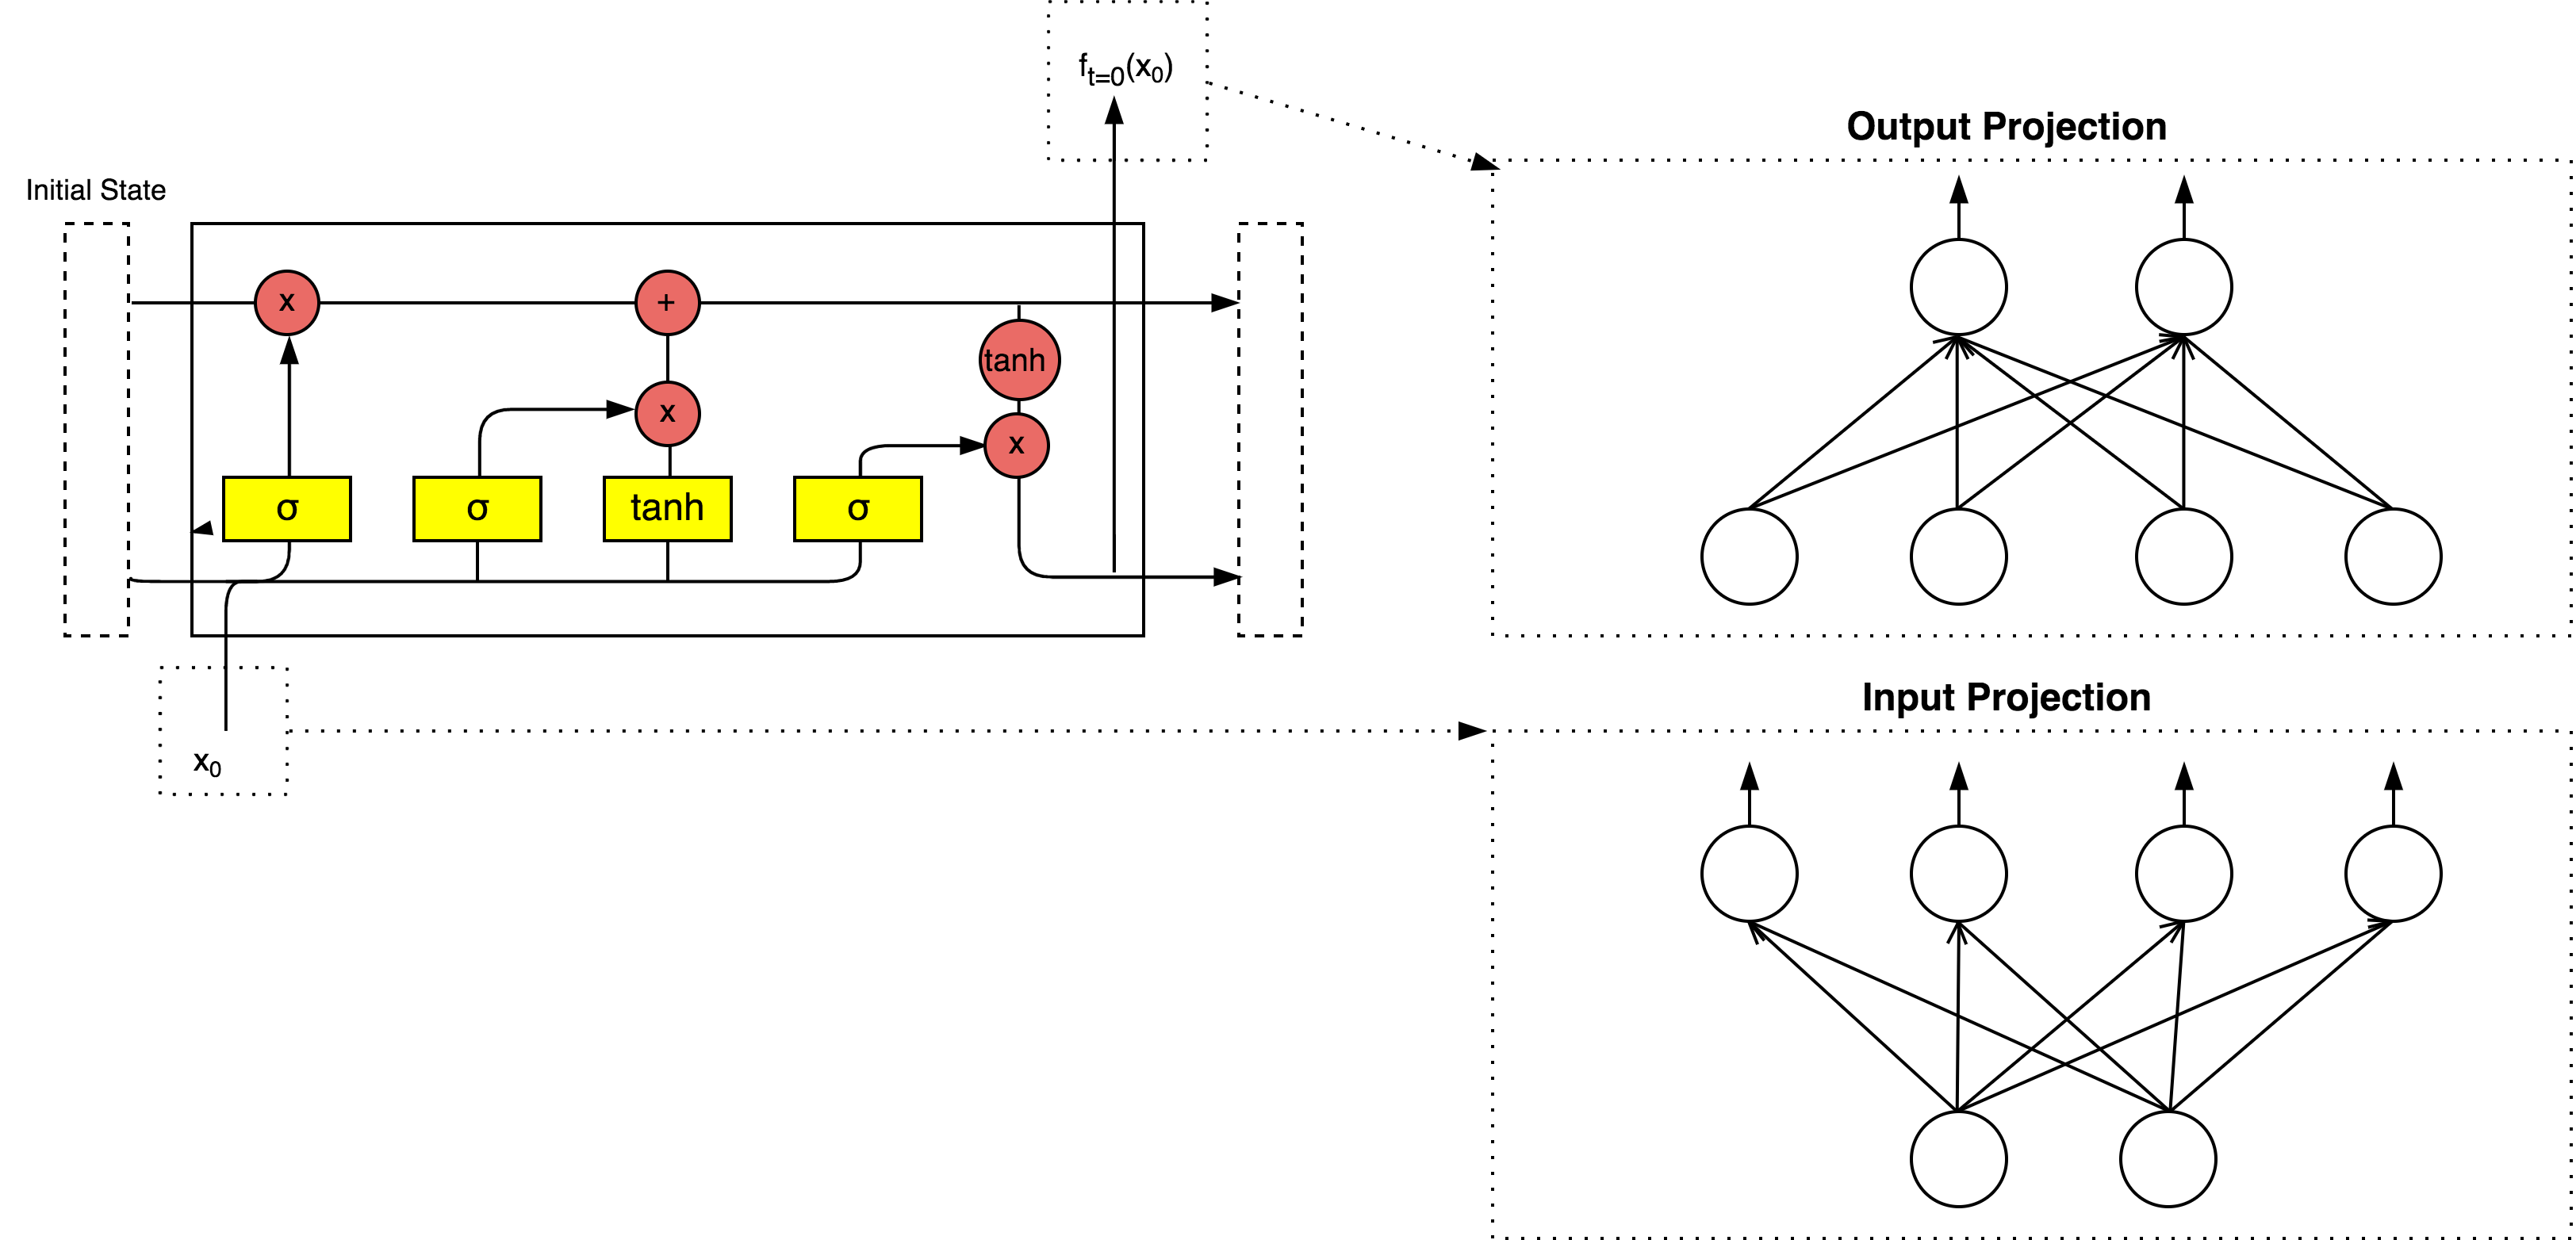
\includegraphics[width=0.7\textwidth]{lstm-projection}
  \caption{Example of projection within a LSTM cell with 4 hidden states.}
  \label{fig:lstm-projection}
\end{figure}

Some of the traces can be particularly long and therefore the network needs to be unrolled to extreme lengths \cite{greschbach2016effect}.
In fact, given memory constraints, this issue can become a major problem.
This can be solved by cutting the traces after a couple seconds since it has been shown that the first part of a trace carries more information than the latter \cite{TODO: Include}.

\begin{figure}[ht]
  \centering
  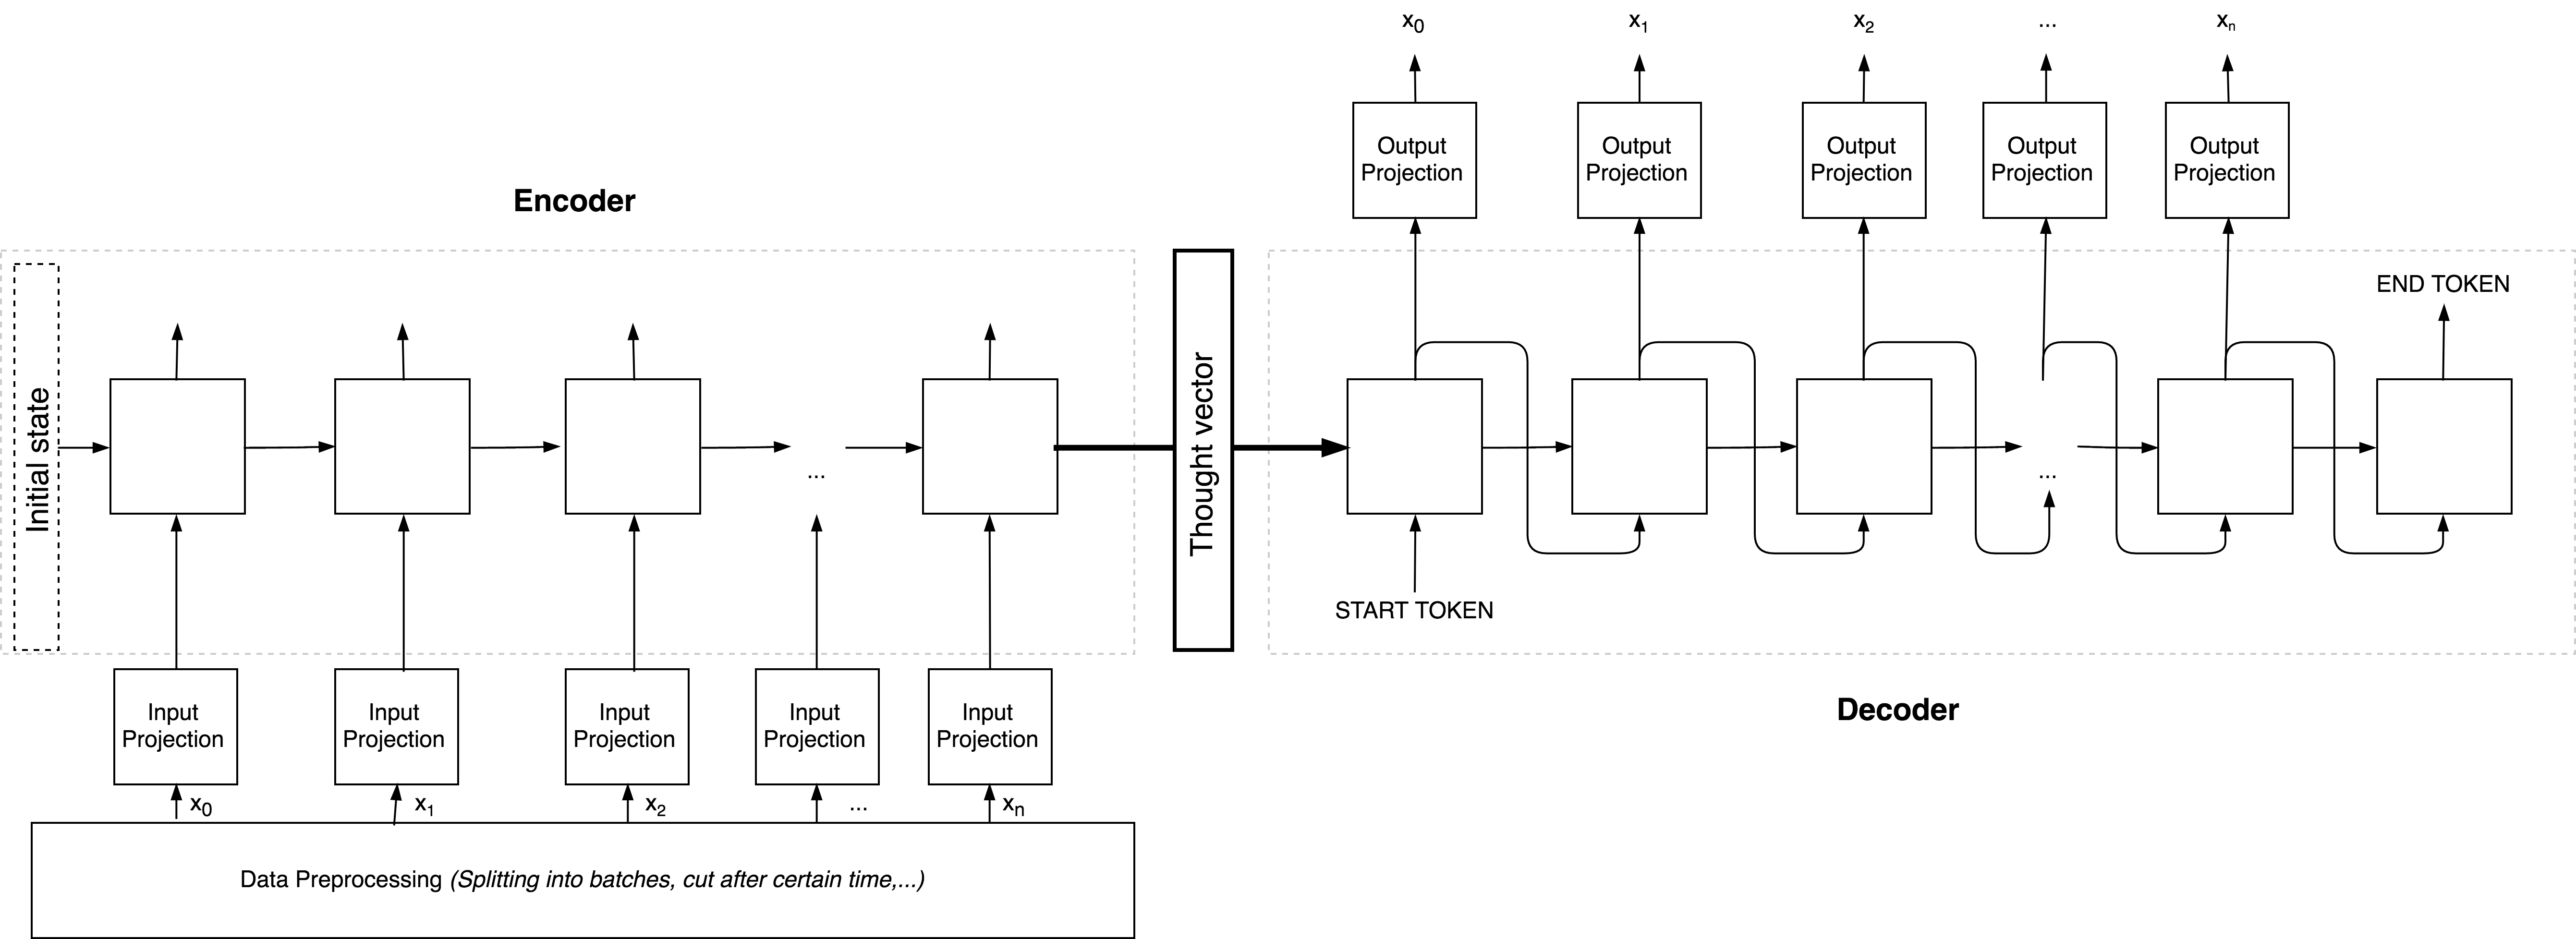
\includegraphics[width=\textwidth]{full-seq2seq}
  \caption{Overal structure of our sequence-to-sequence model.}
  \label{fig:full-seq2seq}
\end{figure}

Based on the above, we can construct our \textit{computational graph} in Tensorflow as outlined in figure \ref{fig:full-seq2seq}.

\section{Attack Strategy}

Here we consider an adversary that relies on deep learning to extract fingerprints for a website fingerprinting attack.
This adversary can have two different goals in mind, as previously stated in section \ref{sec:threat-model}.
In this work, the adversary relies on a sequence-to-sequence to extract the fingerprint from Tor cells for both goals.
The full attack, however, can be split up into four different stages: \textit{data collection}, \textit{fingerprint extraction training}, \textit{classifier training} and \textit{the attack}.
\\\\
\noindent
\textbf{Data Collection}
\begin{enumerate}
  \item Choose web pages that the attacker wishes to monitor.
  \item Collect traffic for a set of monitored sites and unmonitored sites.
  \item Convert the raw TCP data into Tor cells.
  \item Remove SENDMEs and other noise.
\end{enumerate}

\noindent
\textbf{Fingerprint Extraction Training}
\begin{enumerate}[resume]
  \item Further process the data into batches and perhaps cut the data of individual traces after several seconds.
  \item Prepare the sequence-to-sequence model.
  \item Train the sequence-to-sequence model on a copy task for monitored and some unmonitored web pages.
  \item Extract fingerprints from data by using the trained sequence-to-sequence model.
\end{enumerate}

\noindent
\textbf{Classifier Training}
\begin{enumerate}[resume]
  \item Given a classifier, train it using the extracted fingerprints.
  \item Measure performance of classifier.
\end{enumerate}

\newpage

\noindent
\textbf{The Attack}
\begin{enumerate}[resume]
  \item Passively capture traffic from Tor users.
  \item Pre-process the collected data.
  \item Extract fingerprints using the trained sequence-to-sequence model.
  \item Classification via the trained classifier.
\end{enumerate}

\begin{figure}[ht]
  \centering
  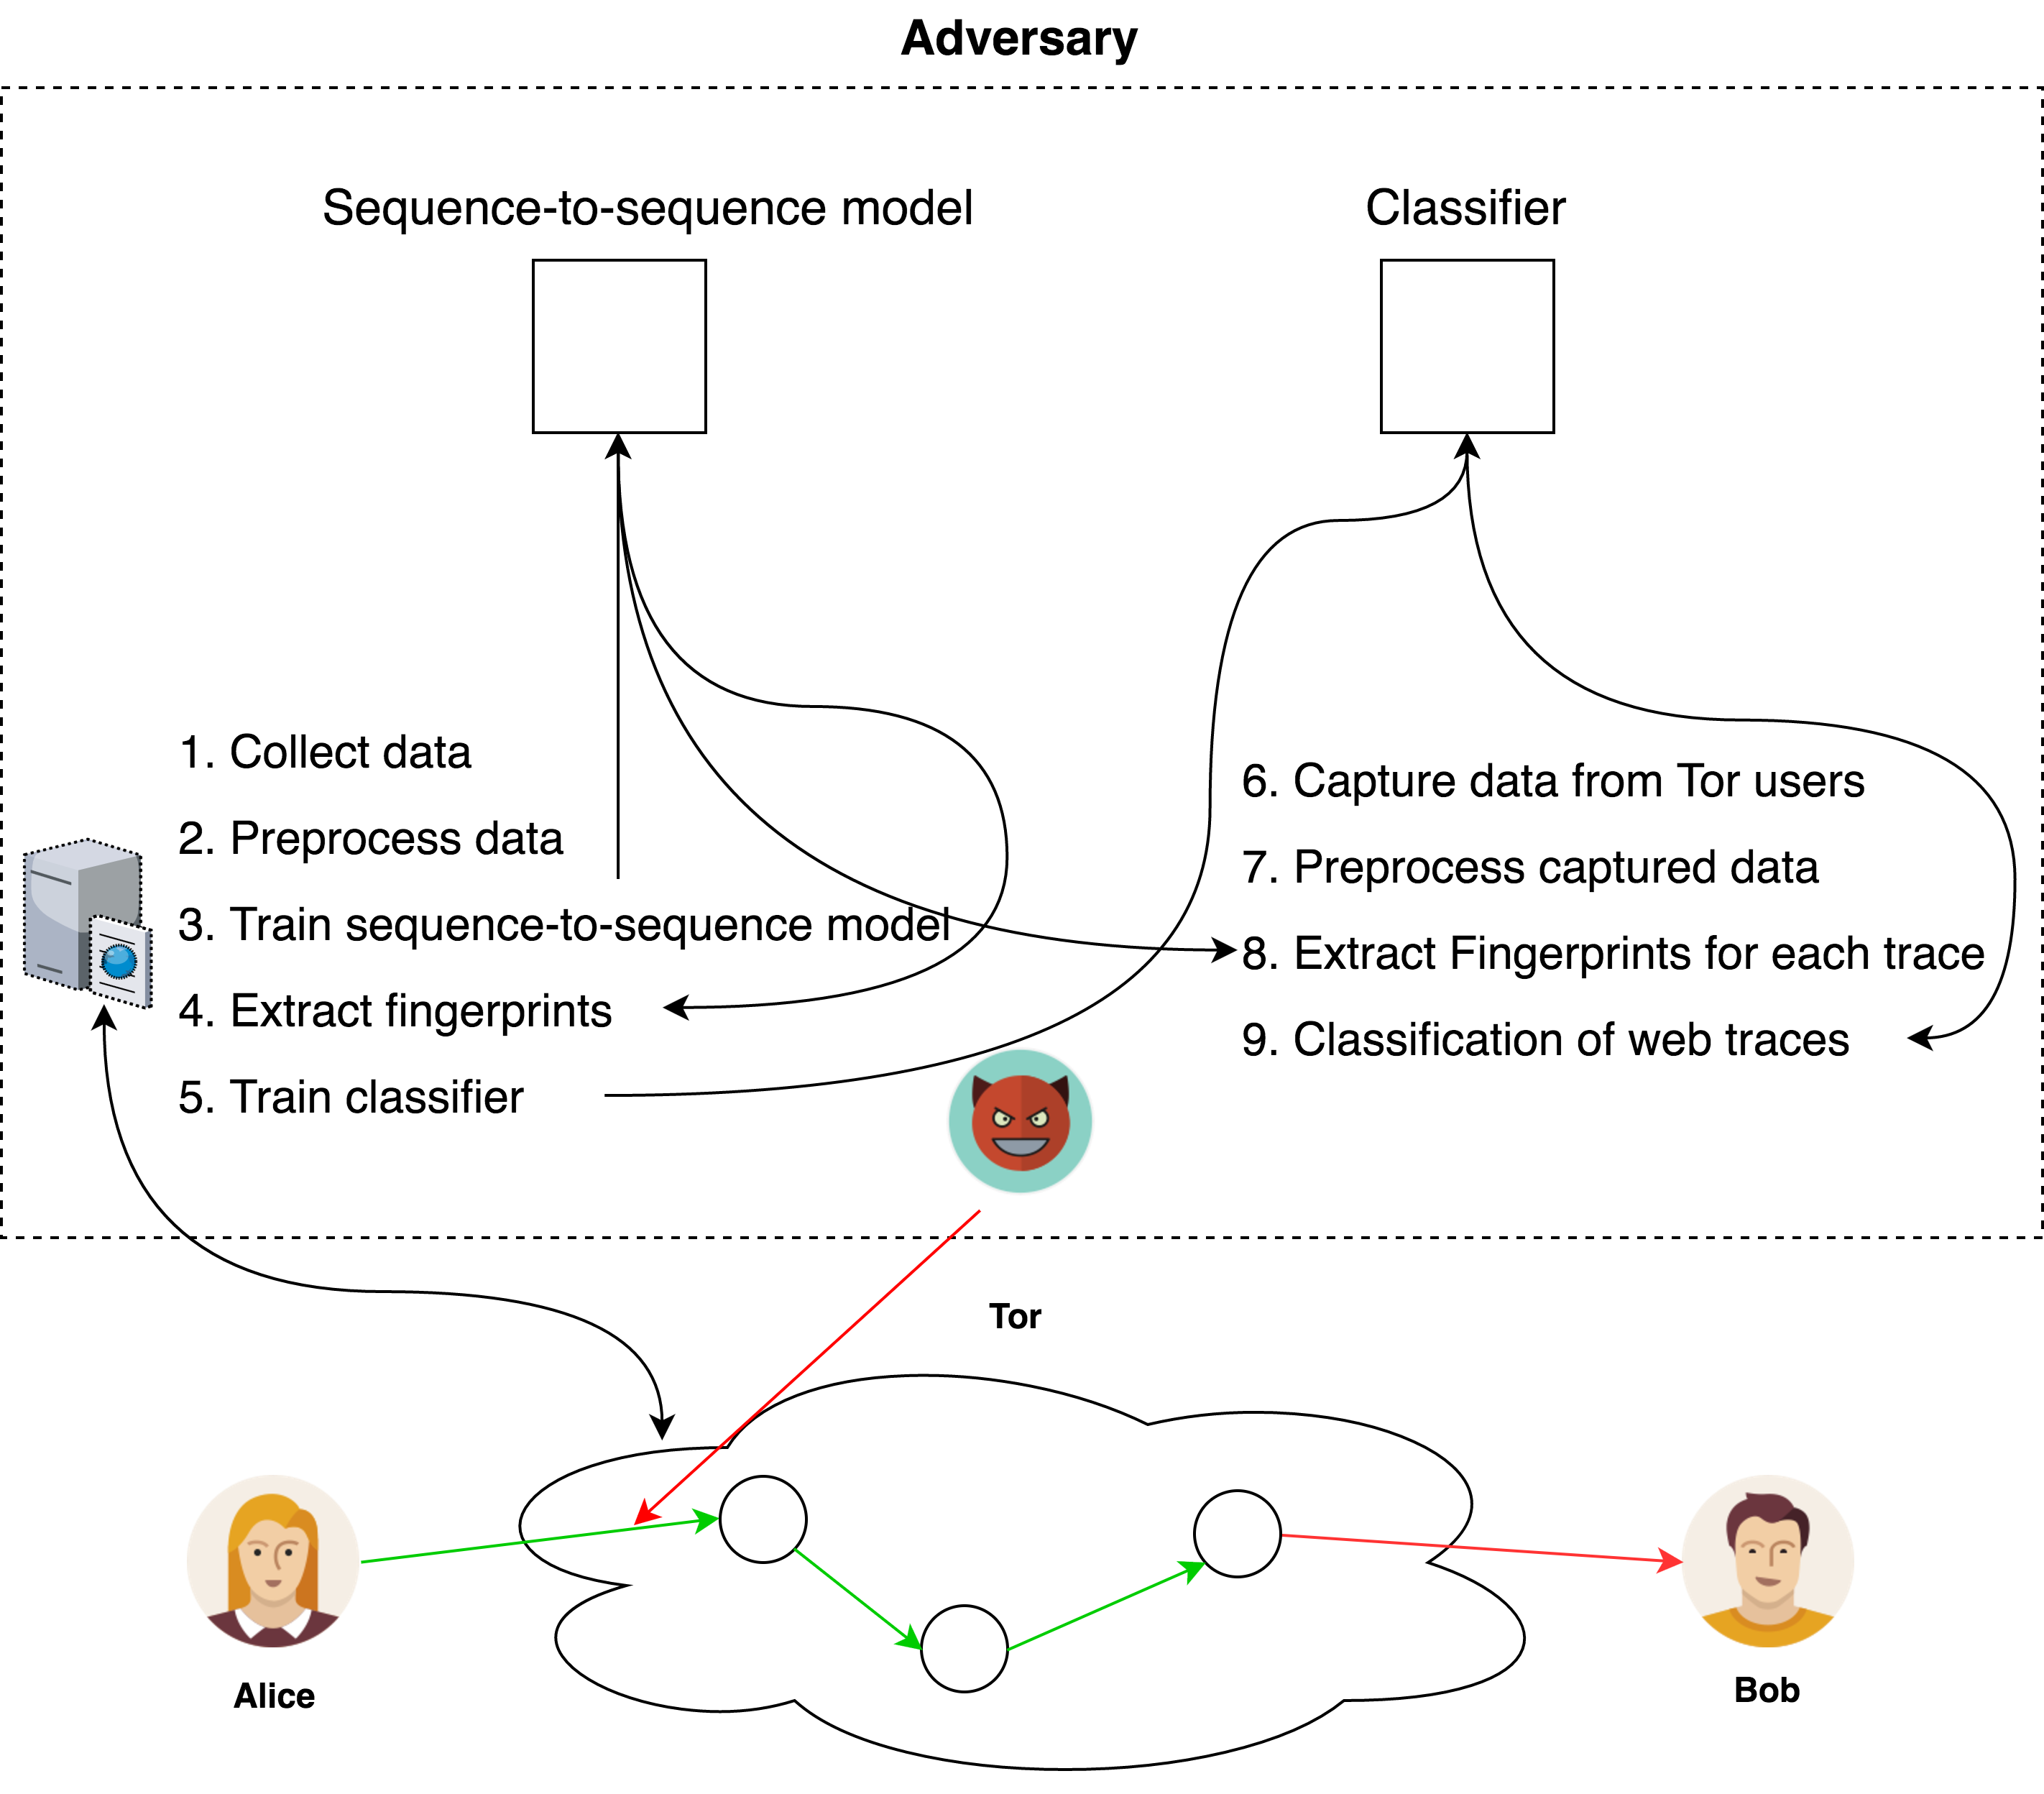
\includegraphics[width=0.7\textwidth]{overall-structure}
  \caption{Attack strategy.}
  \label{fig:attack-strategy}
\end{figure}

\subsection{Data Collection} \label{sec:data_collection1}

As previously mentioned, the data collection process first requires the adversary to choose a set of $n$ websites to monitor.
Next, the adversary crawls these pages a total of $i$ iterations to ensure that a classifier has enough data to generalize.
As suggested by Wang et al. when performing page loads, browser caching should be disabled since Tor does not allow caching to disk and therefore the browser cache is cleared every time it is restarted \cite{wang_goldberg_2013}.
After the collection, the TCP data is converted into Tor cells and probabilistic algorithms are used by Wang et al. \cite{wang_goldberg_2013} to remove SENDMEs.
This data can be processed further, however we chose not to since the model should be able to learn how to perform this processing.

Most of our analysis will be done using the dataset provided by Greschbach et al. \cite{greschbach2016effect}, which can be used for open-world analysis since it provides us with $100$ samples for Alexa's top $9000$ websites and one sample of one sample for $909,000$ unmonitored sites.
For the rest of this paper, we will refer to this dataset as \texttt{GRESCHBACH}.
Next, to see how our model performs on a dataset, whose data is recorded at a different time and under different circumstances, we will also be using the dataset provided by Wang et al. \cite{wang_cai_johnson_nithyanand_goldberg_2014}, which we will call \texttt{WANG14} \cite{panchenko2}.
This set is slightly smaller with $100$ monitored websites with $90$ instances each and $8400$ unmonitored sites.

\subsection{Fingerprint Extraction Training} \label{sec:fingerprint-extraction-training}

In order to truly evaluate the model, we need to split the data up into a training and validation set.
We do not train the model on any data in the validation set but instead use it to see how well the model performs on unseen data.
For this split, we use a \textit{stratified shuffle split}, meaning that we shuffle the data and then perform the split, whilst preserving the class distributions.
On top of training the feature extractor with monitored pages, we also train it on unmonitored pages, as it needs to be able to extract features effectively from both sets.

To gain performance and perhaps even a faster convergence, \textit{mini-batch processing} will be used to train the sequence-to-sequence model.
Each batch can either be presented in \textit{batch-major} or \textit{time-major} form.
Although time-major is slightly more efficient \cite{tensorflow}, we opt for a batch-major form, since it makes the fingerprint extraction easier.

When dividing the data up into batches, we also need to determine how big the batches will be.
The bigger they are, the larger the performance gain will be but the lower the accuracy might be.
Additionally, the size of the batches also depend on the amount of available memory.
Next, after the data has been divided, we perform some further processing such as cutting the traces after several seconds.
Finally, since all of the traces within a batch need to be of the same length, padding is performed as a final preprocessing step.

After collecting and fully preprocessing the data, the adversary can start to construct the sequence-to-sequence model.
However, in order to do so, there are a variety of different architectures that need to be chosen.
Some of which that we will consider are outlined below:

\begin{itemize}
  \item Which sort or RNN cells to use. This can either be a GRU or an LSTM cell.
    We could also potentially investigate the usefulness of multilayered RNN cells but it would make the network even deeper.

  \item Using a bidirectional encoder to ensure that the output at time $t$ is not only affected by past information but also on future information.

  \item The amount of hidden states within a RNN cell, which affects the length of the fingerprints.
\end{itemize}

The adversary woulds like to have the amount of learned features to be small enough.
Since the bigger the amount of features, the more training data is required, due to the \textit{curse of dimensionality}.
However, if the amount of hidden states within a cell is too low, it might not be able to effectively recreate a trace from a fingerprint, due to the lack of data.
Hence, the adversary will need to consider this tradeoff when choosing the model architecture.

Now that the model has been constructed, the adversary still has to chose various learning parameters such as:

\begin{itemize}
  \item The optimizer to use (\textit{adam}, \textit{gradient descent} or \textit{RMSProp}) \cite{tensorflow}.
  \item Learning rate ($\gamma$) for the previously chosen optimizer.
  \item Amount of traces within a single mini-batch ($b$).
  \item Cost, or loss function ($f$) to minimize (\textit{mean squared error} (MSE), \textit{absolute loss} (AL) or \textit{cross-entropy}) \cite{tensorflow}.
  \item Whether or not to reverse the traces. This parameter does not make a difference when using a bidirectional encoder.
  \item After how much time the traces are cut.
\end{itemize}

After these parameters have been tuned, the computational graph can be constructed in Tensorflow and the training can be started using the training data.
When this training has been completed, fingerprints can be extracted for data within the test set.

On top of this, we also often have a small set, called the \textit{validation set}, which is not used for training.
But it is used whilst training, to see how the network performs on unseen data during the training process.

\subsection{Classifier Training} \label{sec:classifier-training}

After the adversary has extracted the fingerprints for websites within the test set, they need to construct a classifier.
This classifier can then use these fingerprints to learn how to classify web pages.
Most works so far rely on some sort of \textit{supervised machine learning} techniques such as \textit{support vector classifiers} (SVC), \textit{k-nearest neighbours} (kNN), \textit{random forests} (RF) or \textit{naive bayes} (NB) \cite{panchenko1,panchenko2,wang_cai_johnson_nithyanand_goldberg_2014,kfingerprinting,naivebayes}.
All of these algorithms rely on different techniques but an explanation of their inner workings is outside the scope of this paper.
Instead, we will consider them as \textit{black box} models.
This means that all we know is that we can apply a \texttt{fit} function to the models, which causes them to learn how to classify the fingerprints and a \texttt{predict} function, which predict the class of given inputs.
However, in reality, an adversary will have to carefully consider which models to use and tune the hyperparameters of that specific model to get the best possible performance.

To measure the performance of our black-box models, we use a similar technique as we did in the previous section.
We split our test set up into two more sets, a \textit{classifier training set} and a \textit{classifier test set}.
But since training a classifier, requires less time, we can use another technique, called \textit{stratified k-fold validation}.
Here we split our original test set up into $k$, mutually exclusive, folds.
Next, one of the folds is chosen to be the classifier test set and all of the other folds form the classifier training set.
This process is repeated for $k$ iterations, where for each iteration, a different fold is chosen to be a test set.
However, what is special about stratified k-fold validation is that the class distributions are preserved within the folds.

\begin{figure}[ht]
  \centering
  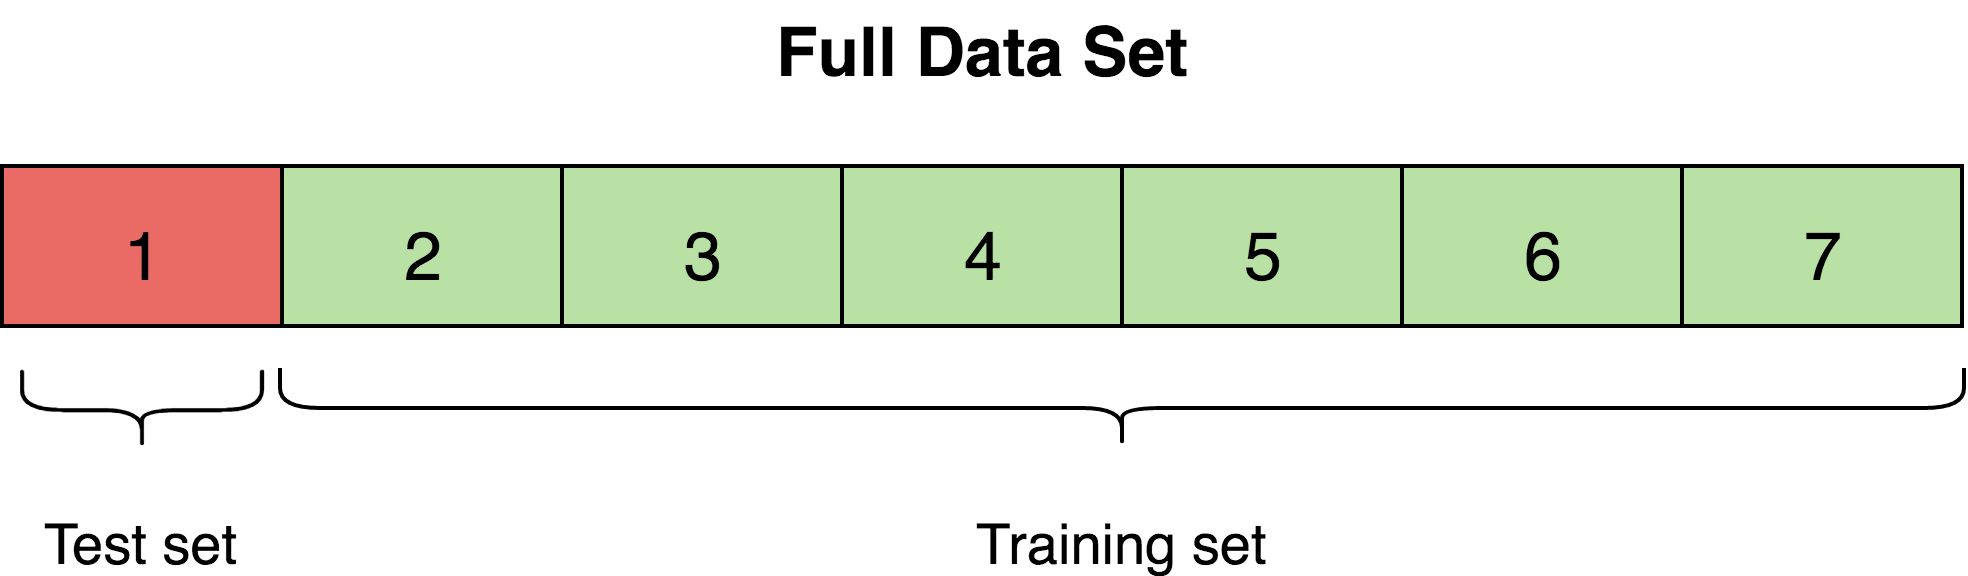
\includegraphics[width=0.6\textwidth]{kfold}
  \caption{Example of one iterations in a k-fold validation $(k = 7)$.}
  \label{fig:kfold}
\end{figure}

For each iteration of the validation process, several statistics can be recorded and then averaged over all iterations.
This process ensures that every data point will be in the test set at least once and therefore giving us an accurate measure of these statistics.

Some of the statistics that are used for the performance measure of models, are outlined below within the context of a website fingerprinting attacks:
\begin{itemize}
  \item \textbf{True Positive Rate (TPR)} is the probability that a monitored page is classified as the correct monitored page \cite{kfingerprinting}.

  \item \textbf{False Positive Rate (FPR)} is the probability that an unmonitored page is incorrectly classified as a monitored page \cite{kfingerprinting}
    (Often TP, FP, together with false negative (FN) and true negatives (TN) are combined together into what is called a \textit{confusion matrix}).

  \item \textbf{Bayesian Detection Rate (BDR)} is the probability that a page corresponds to the correct monitored page, given that the classifier recognized it as that monitored page \cite{kfingerprinting}.
    This can be calculated as follows:
    $$\text{BDR} = \frac{\textit{TPR} \times \Pr(M)}{\textit{TPR} \times \Pr(M) + \textit{FPR} \times \Pr(U)}$$
    where
    $$\Pr(M) = \frac{|\text{Monitored}|}{|\text{Total Pages}|}, \quad \Pr(U) = 1 - \Pr(M)$$

    This measure essentially indicates the practical feasibility of the attack, as the adversary is mainly concerned with this specific measure \cite{kfingerprinting}.

  \item \textbf{Accuracy (A)} is the percentage of correctly classified instances.
    Although it can be used as a rough indicator, it will not be used in the final conclusions because of the \textit{accuracy paradox}, which arises due to class imbalance.

  \item \textbf{F1-Score (F1)} measures the harmonic mean between precision and recall \cite{scikitlearn}.
    \begin{align*}
      \text{F1} &= 2 \times \frac{\text{precision} \times \text{recall}}{\text{precision} + \text{recall}}\\
                &= \frac{2 \times \textit{TP}}{2 \times \textit{TP} + \textit{FP} + \textit{FN}}
    \end{align*}
    where
    $$\text{recall} = \frac{\textit{TP}}{\textit{TP} + \textit{FN}}, \quad \text{precision} = \frac{\textit{TP}}{\textit{TP} + \textit{FP}}$$

    This measure is particularly useful since it is not affected by class imbalance.
\end{itemize}

Rather than using another classifier, we could also potentially add a \textit{softmax layer} on top of our encoder, like V. Rimmer uses on top of her stacked autoencoder \cite{deeplearningthesis}.
This process would involve first training the sequence-to-sequence model, then stacking the softmax layer on top of each unrolled cell in the encoder and using it for classification.
What would be interesting about this approach is that the adversary can analyse how the probability of a trace being classified changes, as it analyses packets from the trace.
However, this is outside the scope of this paper, as we are focusing on the feature extraction process.

\begin{figure}[ht]
  \centering
  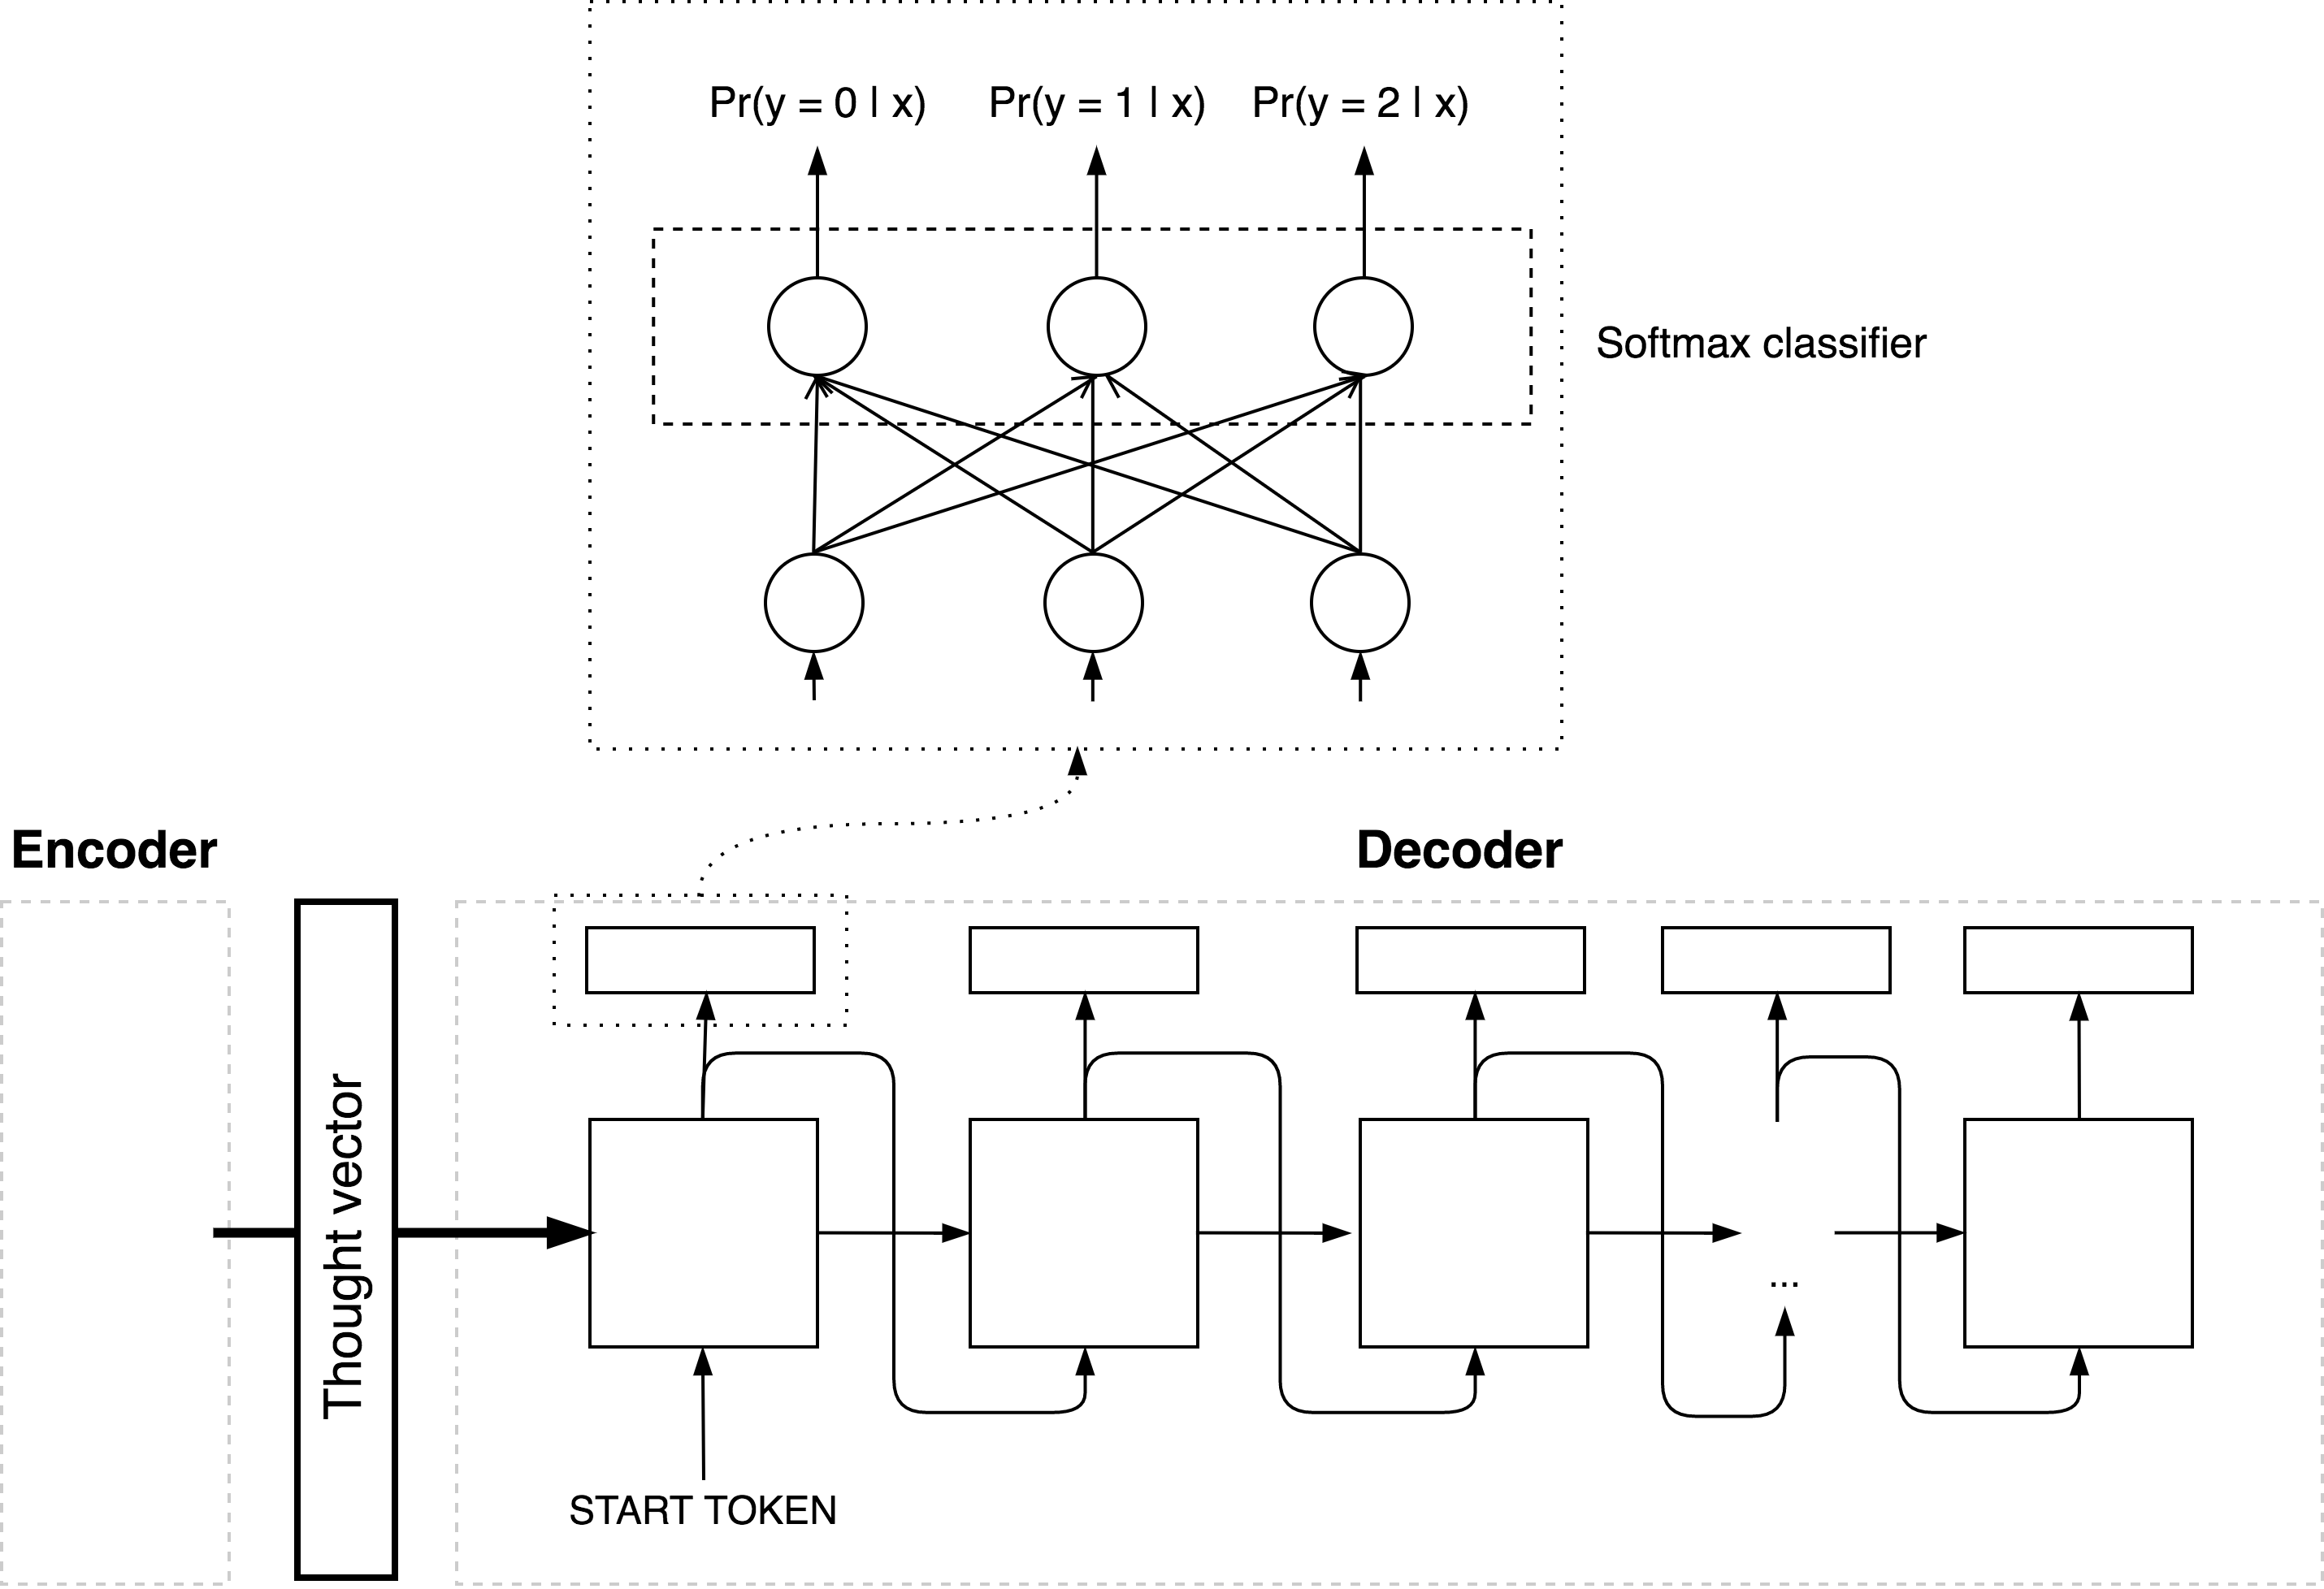
\includegraphics[width=0.6\textwidth]{softmax}
  \caption{Example of encoder with softmax layer for 3 web pages.}
  \label{fig:softmax}
\end{figure}

\newpage

\subsection{The Attack}

Finally, after the adversary has trained the required models, the real WF attack can start.
First, the adversary starts capturing web traffic data between the user and the first Tor node, as shown in figure \ref{fig:threat_model}.
Next, the data is processed for the fingerprint extraction process, as described in section \ref{sec:fingerprint-extraction-training}.
After all processing has been done, fingerprints are extracted using the previously trained sequence-to-sequence model.
Finally, those fingerprints are used as features for a classifier, which classifies which web pages the adversary is visiting.

The time between data collection for training and performing the WF has to be kept as small as possible since Juarez et al.'s experiments show that website's content changes greatly over time, therefore affecting the accuracy of the attack \cite{wfpevaluation}.

\section{Code Structure}

In the work, we will not be conducting the final stage of a WF attack.
Instead, we will be reporting the results on the test sets.
All of this is reflected in the overall structure of the code, which consists of four main components, as can be seen in figure \ref{fig:code-structure}.

\begin{figure}[ht]
  \centering
  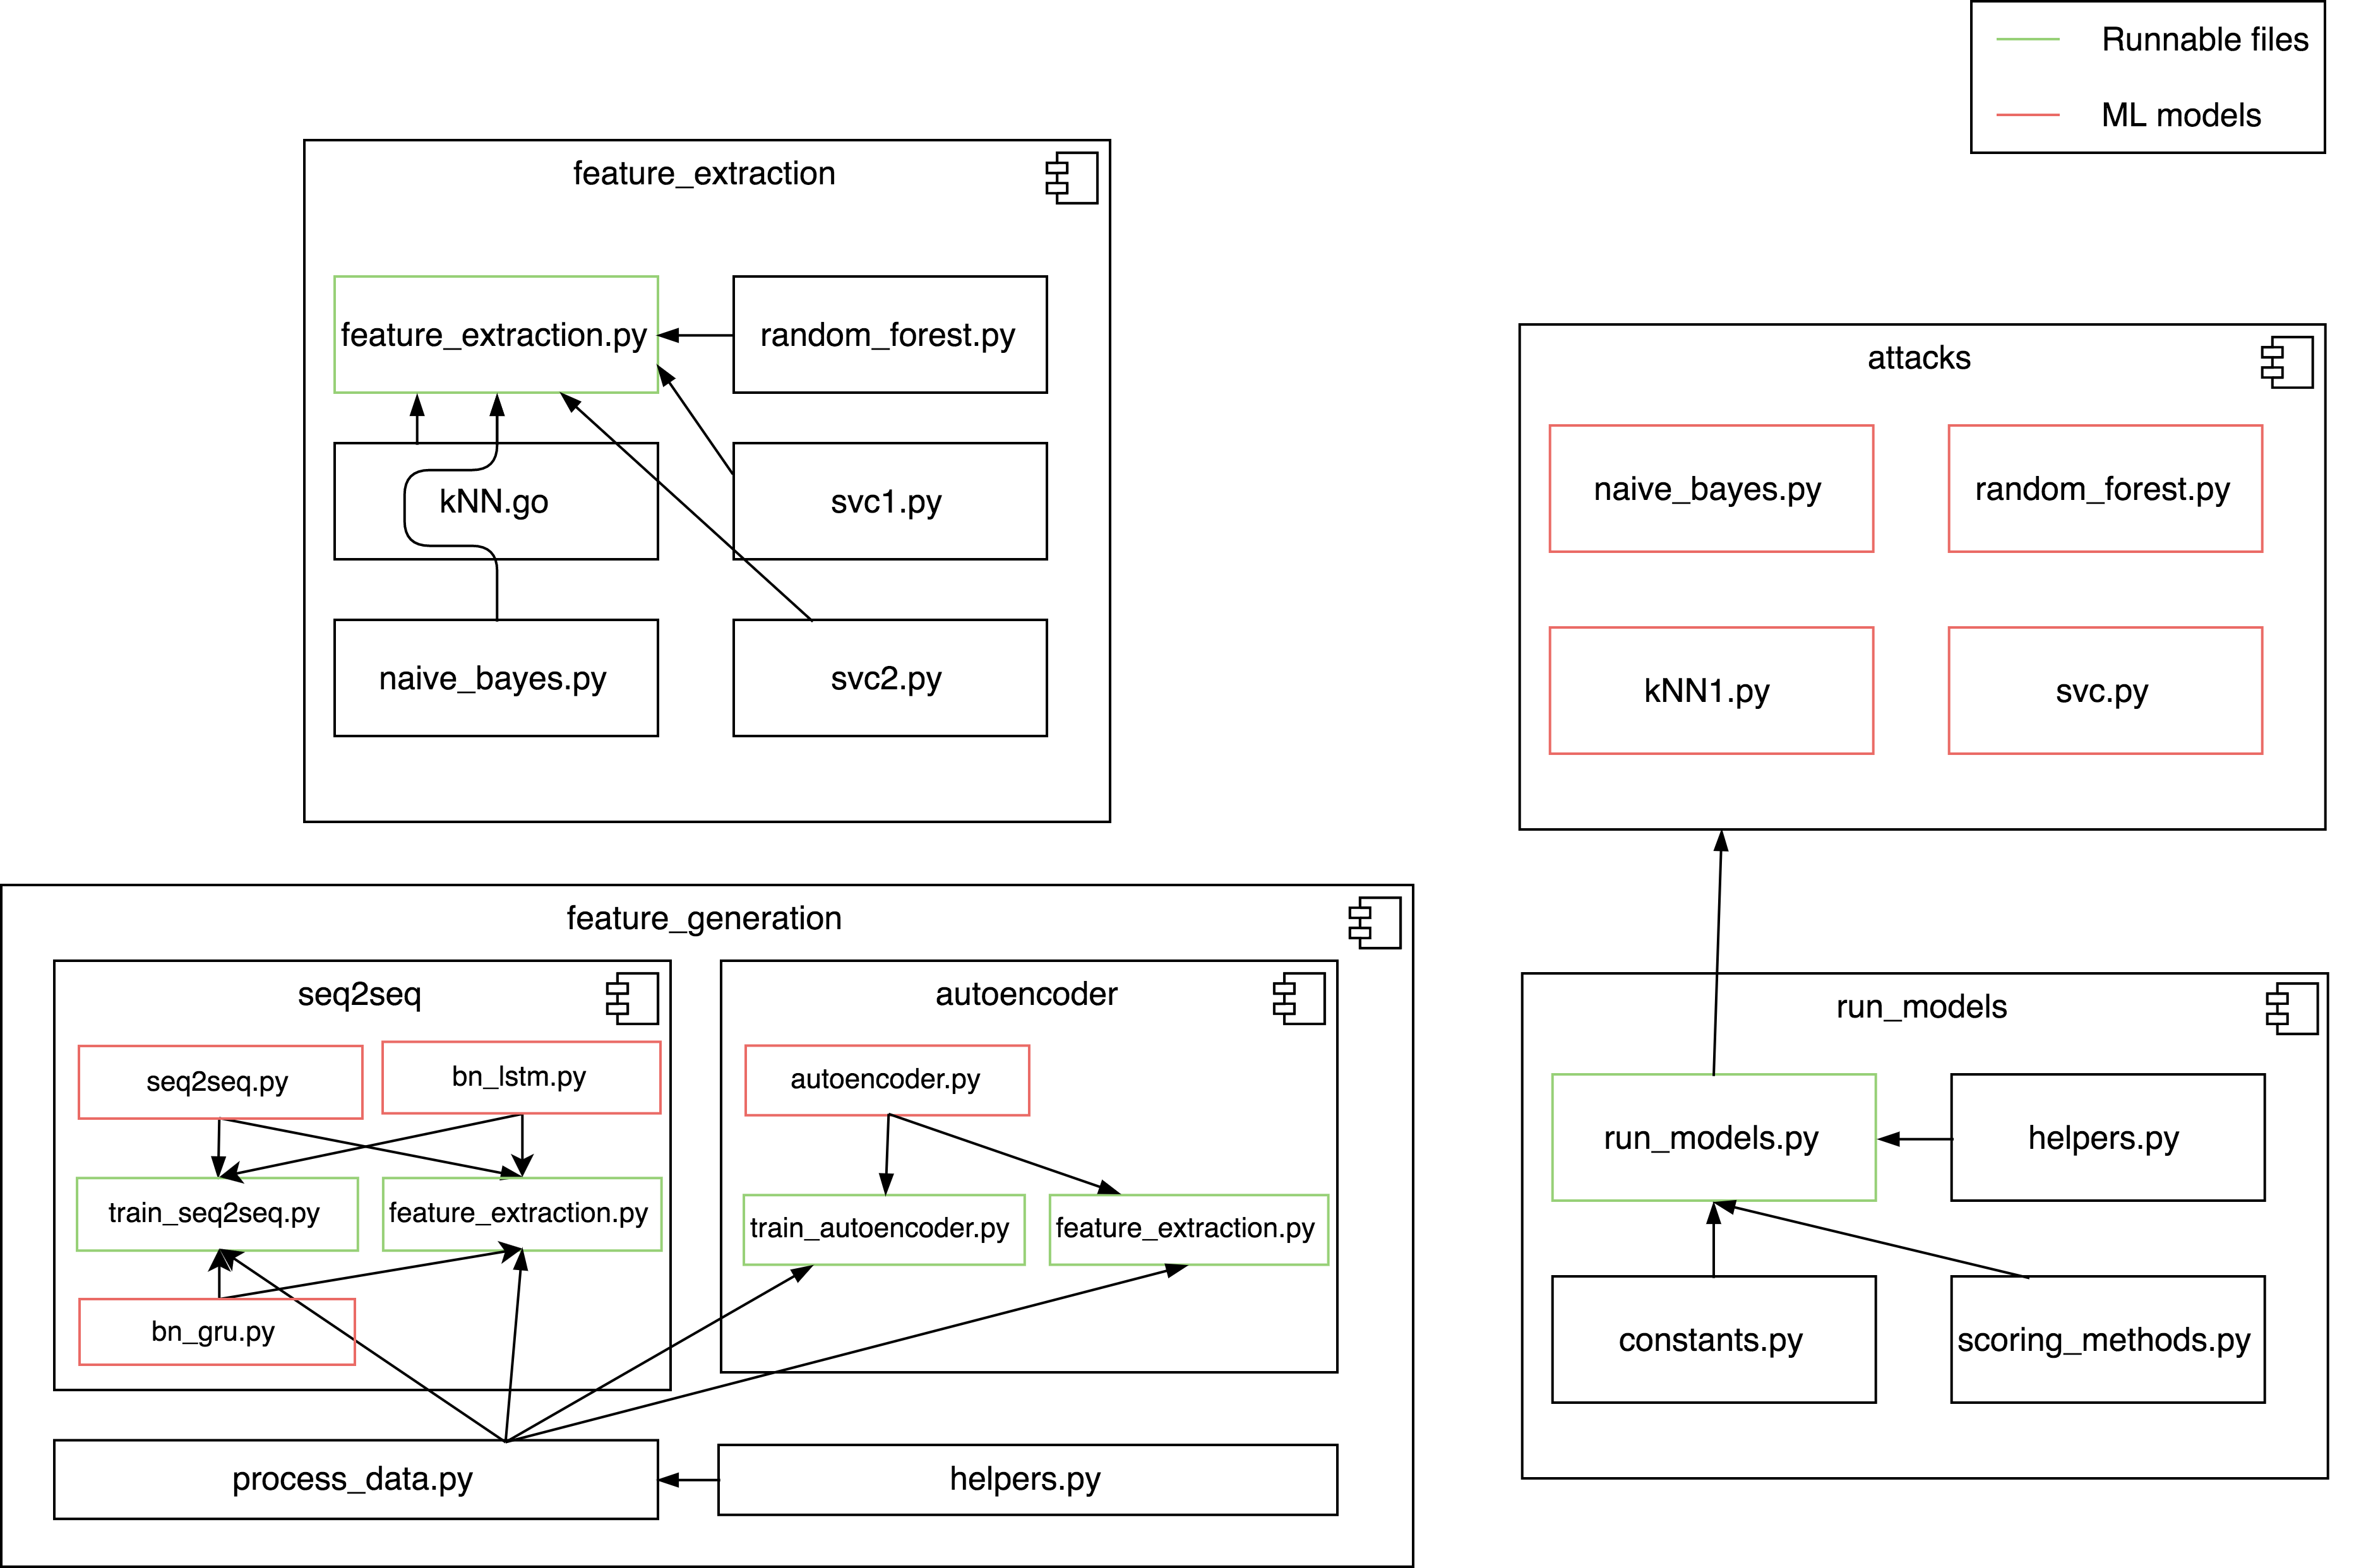
\includegraphics[width=0.6\textwidth]{code-structure}
  \caption{Diagram of how different components are related.}
  \label{fig:code-structure}
\end{figure}

All of the data that is used within this work has already been preprocessed, as described in section \ref{sec:data_collection1}.
The \texttt{feature\_generation} module contains all of the code to further preprocess the data, train the sequence-to-sequence model defined in \texttt{new\_model.py} and to extract the fingerprints using that new model.

All of the models that will be used for the attack section are defined in the \texttt{attacks} module.
We tried to pick a variety of models used, to measure how our fingerprints work on different models.
The logic to actually run the models is defined in the \texttt{run\_models} module, which also does some data preprocessing and defines the logic for the stratified k fold validation and the different scoring methods.

Finally, there is also the \texttt{feature\_extraction} module, whose use will be explained later.

As can be seen, all of the code is written in Python, due to the wide availability of machine learning tools.
Except for the \texttt{kNN.go} file, in the \texttt{feature\_extraction} module, which is written in \textit{Golang} to gain a performance boost \cite{gokNN}.
